\documentclass{article}
\usepackage[left=3cm, right=3cm, top=3cm]{geometry}
\usepackage{bm}
\usepackage[utf8]{inputenc}
\usepackage{ amssymb }
\usepackage[dvipsnames]{xcolor}
\usepackage{fancyhdr}
\usepackage{indentfirst}
\usepackage{amsmath}
\usepackage{titlesec}
\setcounter{secnumdepth}{4}
\pagestyle{fancy}
\fancyhf{}
\cfoot{\thepage}
\rhead {Dominika Bakalarz}

\title {General Linear Model - Apple data}
\author{Dominika Bakalarz}
\date{}

\usepackage{natbib}
\usepackage{graphicx}

\begin{document}

\maketitle

\section{Introduction}
This report presents an analysis of “Apple” data concerned with the growth of Alicyclobacillus Acidoterrestris CRA7152 in Apple Juice. Its goal is to determine factors affecting the presence of CRA7152 growth. Following factors were measured during the experiment: pH level, Brix level (sugar content), the temperature of the juice and Nisin level (food preservative), 74 data samples were obtained. \\


\section{Exploratory Data Analysis}
There are four potentially explanatory variables available: ph, brix, temperature, nisin. All variables are continuous. 

As we can see in Figure 1, CRA7152 Growth is present more often in samples with high pH level, low Nisin level, medium level temperature and low Brix level. These conclusions will be explored further and verified by suitable experiments in the next part of the report. 
\begin{figure}[h!]
\centering
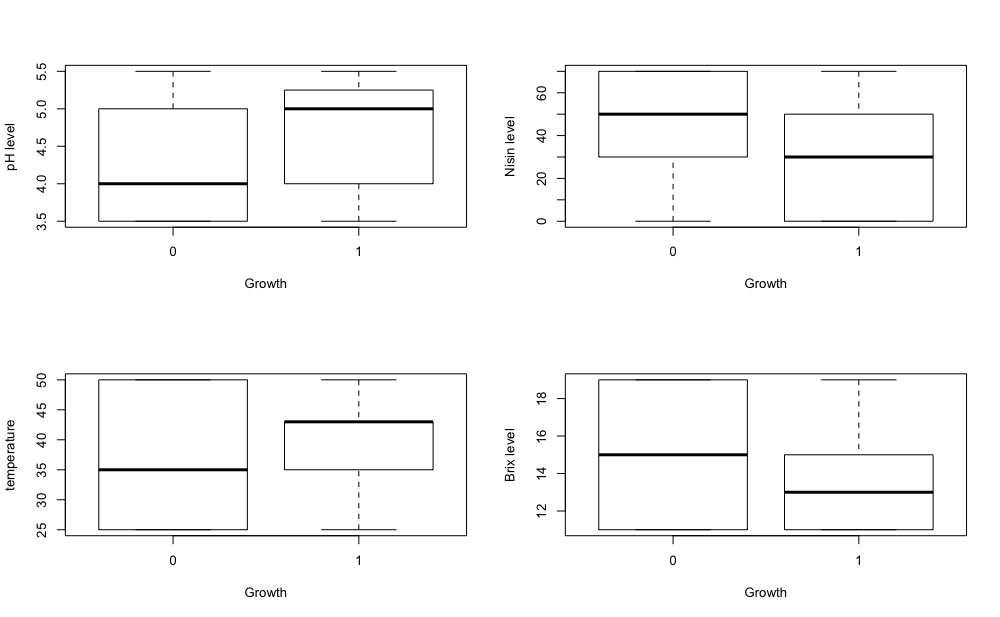
\includegraphics[scale = 0.35]{boxplots.png}
\caption{Boxplots presenting the dependence between CRA7152 growth (0 - absent, 1 - present) and each explanatory variable}
\end{figure}
\\

We have checked that in 32 samples growth is present, and in the remaining 42 samples it is absent, so we have balanced data. Therefore, when plotting Figure 2, we decide to scale the data, so that the heights of red and blue  bars  represent percentages of all samples with growth present and absent, respectively. That is, in each of the four plots in Figure 2, all blue bars add up to 1 and all red bars add up to 1. Plots in Figure 2 confirm the conclusion drawn from the boxplots in Figure 1. Moreover, we can see that each explanatory variable has four levels, and approximately a quarter of all samples can be found at each level, so the data set is balanced with respect to all variables.  



\begin{figure}[h!]
\centering
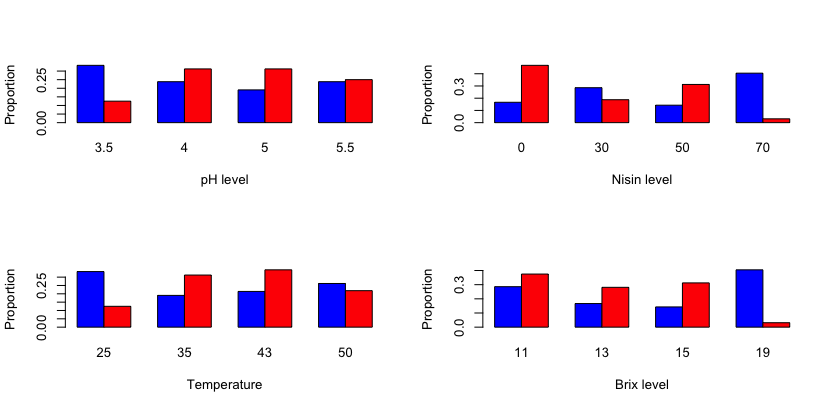
\includegraphics[scale = 0.5]{proportions.png}
\caption{Bar plots presenting growth against each of the explanatory variables. Blue bars represent samples no growth while red bars represent samples with growth present. On each plot, both red and blue bars add up separately to 1. }
\end{figure}

\section{Analysis of the Data}

\subsection{Univariate logistic regression}
\subsubsection{pH level}
We performed univariate logistic regression for each of the explanatory variables, starting with the pH level, with the canonical link function. Now if for $i = 1, 2, ..., 74$  $y_i=$growth$[i] $ and  
$ \boldsymbol{x_i}=(1,$ph$[i]) $
(so we have an intercept and pH level), then we model $y_{i} \sim$   Bernoulli($\pi_i$) with $\pi_i$ the probability of growth present, as a function of pH level. The observation model for $y_i$ has the following probability mass function:
$$ 
f(y_i|\theta_i,\psi)=\pi_i^{y_i}(1-\pi_i)^{1-y_i}= \exp(y_{i}\log(\pi_i/(1-\pi_i))+\log(1-\pi_i))
$$
so $\theta_i=\log(\pi/(1-\pi)$ is the natural parameter, $\psi=1$, $\kappa(\theta_i = \log(1+e^{\theta_i})$ and $c=0$. We have $\mu_i=E(Y_i)=\pi_i$ and the linear predictor is $\eta_i=\beta_1+\beta_2x_{i,2}$. We decide to use the logistic link (which is the canonical link in this case): 
$$
\log(\mu_i/(1-\mu_i))=\eta_i
$$
Thus the probability of growth being present is a logistic function of pH level. 
\\We fit this model to the data. 

\begin{table}[h!]
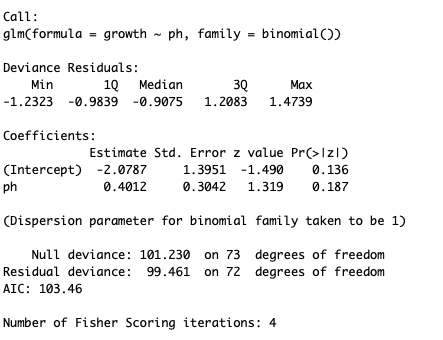
\includegraphics[scale = 0.5]{table1.png}
\caption{Summary of the model growth $\sim$ ph}
\end{table}

As we can see in Table 1, the p-value for the pH level is 0.187, so it is not significant. 
The estimated change in the log odds when we include the ph term is $\overset{\wedge}{\beta_2} $ = 0.4012, what which is an increase of a factor of exp(0.4012) $\backsimeq $ 1.49.
\subsubsection{Brix level}
Now we modify the model by writing $ \boldsymbol{x_i}=(1,brix[i]) $, so the probability of growth being present is now a logistic function of Brix level. We fit this new model to the data. 

\begin{table}[h!]
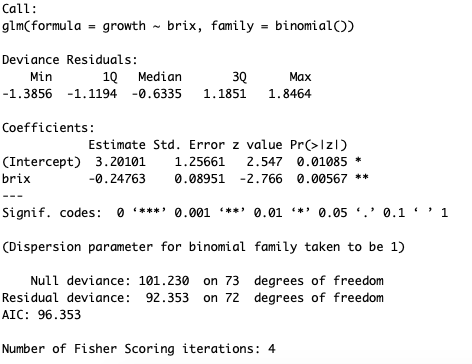
\includegraphics[scale = 0.5]{table4.png}
\caption{Summary of the model growth $\sim$ brix}
\end{table}

As we can see in Table 2, the p-value for the Brix level is 0.00567, so it is very significant (at 5\% significance level). The estimated change in the log odds when we include the brix term is $\overset{\wedge}{\beta_2} $ = -0.24763, what which is an increase of a factor of exp(-0.24763) $\backsimeq $ 0.78.
\subsubsection{Temperature}
We modify the model again by writing $ \boldsymbol{x_i}=(1,temp[i]) $, so the probability of growth being present is now a logistic function of the temperature. We fit this new model to the data. 

\begin{table}[h!]
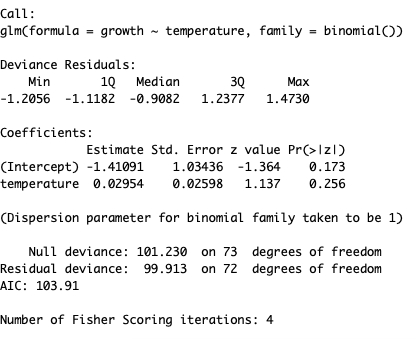
\includegraphics[scale = 0.5]{table3.png}
\caption{Summary of the model growth $\sim$ temp}
\end{table}

As we can see in Table 3, the p-value for the temperature is 0.256, so it is not significant.
The estimated change in the log odds when we include the temperature term is $\overset{\wedge}{\beta_2} $ = 0.02954, what which is an increase of a factor of exp(0.02954) $\backsimeq $ 1.02.
\subsubsection{Nisin level}
We modify the model again by writing $ \boldsymbol{x_i}=(1,nisin[i]) $, so the probability of growth being present is now a logistic function of Nisin level. We fit this new model to the data. 

\begin{table}[h!]
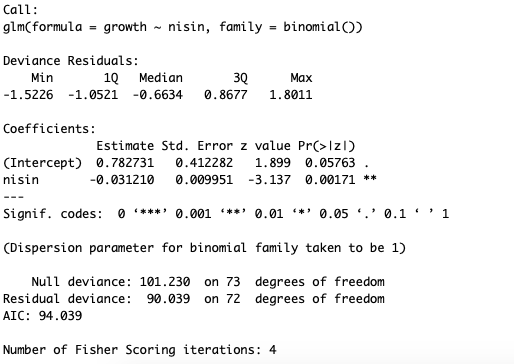
\includegraphics[scale = 0.5]{table2.png}
\caption{Summary of the model growth $\sim$ nisin}
\end{table}

As we can see in Table 4, the p-value for the Nisin level is 0.00171, so it is very significant (at 5\% significance level). The estimated change in the log odds when we include the nisin term is $\overset{\wedge}{\beta_2} $ = -0.03121, what which is an increase of a factor of exp(-0.03121) $\backsimeq $ 0.97.

To summarize, we have found that Brix and Nisin level are very significant explanatory variables, while pH level and temperature are not significant at all (but their interactions with other terms might be significant and also they might become significant in more complex models, we will explore this in the next part of the report).  

\subsection{Model selection}
We will use the GLM set up from the previous section, but we will vary the design matrix X, in order to find the best model.
We start with fitting a full model with four-way interactions (and lower order terms): 
\\(M1)   growth $\sim$ ph : brix : temperature : nisin 
\begin{table}[h!]
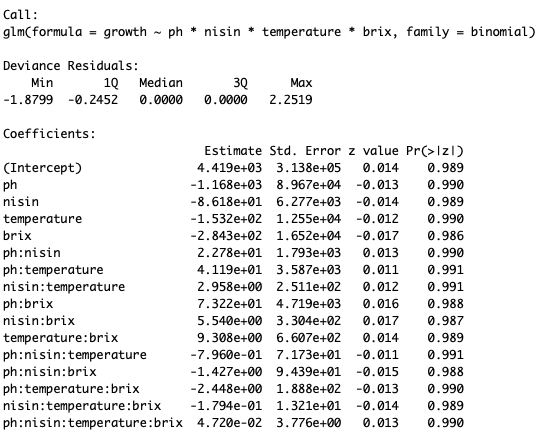
\includegraphics[scale = 0.5]{table5.png}
\caption{Summary of the model (M1) }
\end{table}
\\ We received a warning message saying "glm.fit: fitted probabilities numerically 0 or 1 occurred", which means that the model has over fit and made some dangerous extreme assumptions. This conclusion is confirmed by the model summary shown in Table 5. All p-values are in the range 0.98-1.00 and the coefficient estimates are extremely small. We decide to ignore this model, as it is not feasible. \\ 

We try fitting a model with all three-way interactions (and lower order terms): 
\\(M2)   growth $\sim$ ph : brix : temperature + ph : brix : nisin + ph : nisin : temperature + nisin : brix : temperature
\begin{table}[h!]
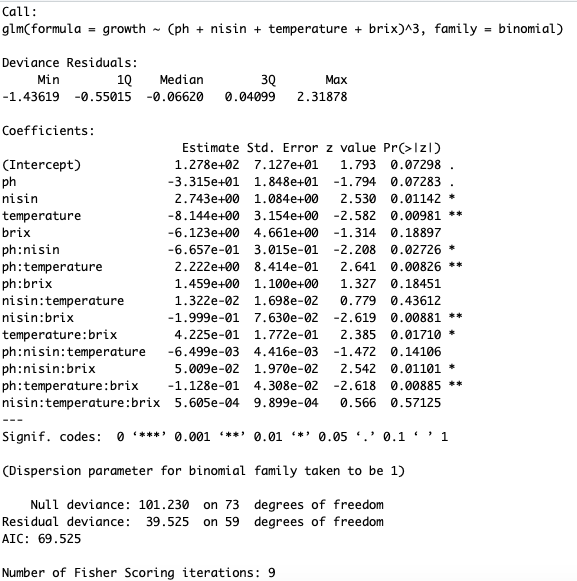
\includegraphics[scale = 0.5]{table6.png}
\caption{Summary of the model (M2) }
\end{table}
\\We again get the same warning, and the estimates are again extremely small, but the p-values look much better now (the summary is presented in Table 6). However, we probably can drop some terms from this model. \\

We try fitting a model with all two-way interactions (and lower order terms): 
\\(M3) growth $\sim$ ph : brix + ph : temperature + ph : nisin + brix : nisin + nisin : temperature + brix : temperature\\
\begin{table}[h!]
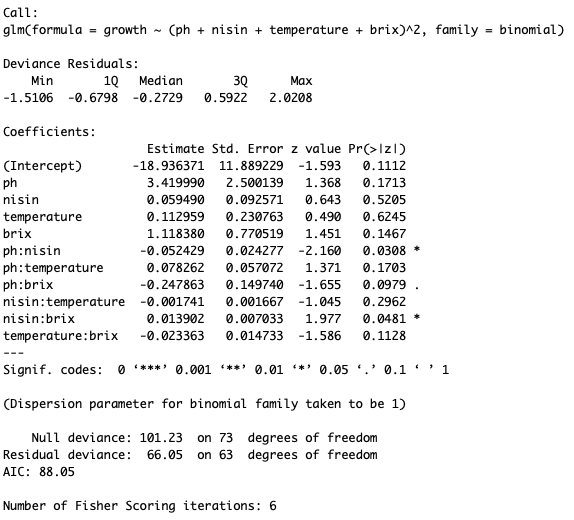
\includegraphics[scale = 0.5]{table7.png}
\caption{Summary of the model (M3) }
\end{table}

We will use the likelihood ratio test to compare the last two models. Model (M2) has deviance 39.525  and 59  degrees of freedom (Table 6), while model (M3) has deviance 66.05 and 63  degrees of freedom (Table 7). So we test 66.05 - 39.525 against chi-squared distribution with 4 degrees of freedom, the p-value is $2.479506*10^{-5}$, so we have to reject model (M2).  

By inspecting the summary of model (M2) we notice that none of the terms nisin:temp, nisin:temp:ph, nisin:temp:brix is significant, so we decide to remove nisin:temp interaction from the model. That is, we are fitting the following model  (including lower order terms):
\\(M4)   growth $\sim$ ph : brix : temperature + ph : brix : nisin \\
\begin{table}[h!]
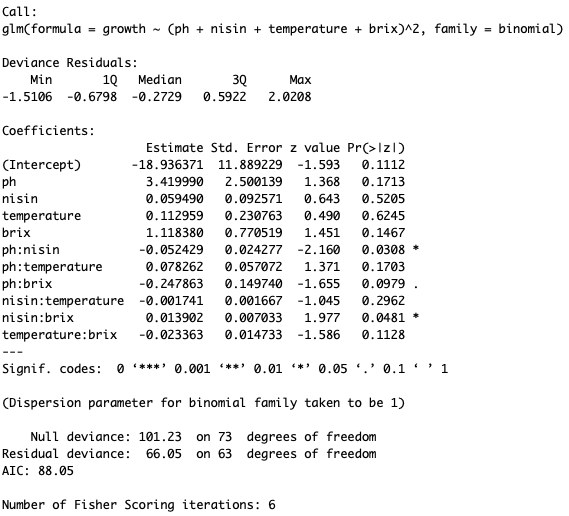
\includegraphics[scale = 0.5]{table8.png}
\caption{Summary of the model (M4) }
\end{table}

We will use the likelihood ratio test to compare (M2) and (M4). Model (M4) has deviance 45.517  and 62  degrees of freedom (Table 8), so we test the LRT statistic 45.517-39.525 against chi-squared distribution with 3 degrees of freedom, the p-value is 0.11, so it is not significant, therefore there is no evidence against model (M4). 

By inspecting the summary of model (M4) presented in Table 8 we notice that the only terms that are not significant (at 5\% significance level) are intercept, brix, ph and ph:brix, but ph:brix:temp and ph:brix:nisin are significant, therefore we cannot simplify this model further, and we choose (M4) as our final model for now. 


\subsection{Goodness of fit}
The goodness of fit test is not applicable to Bernoulli models.
\begin{figure}[h!]
\centering
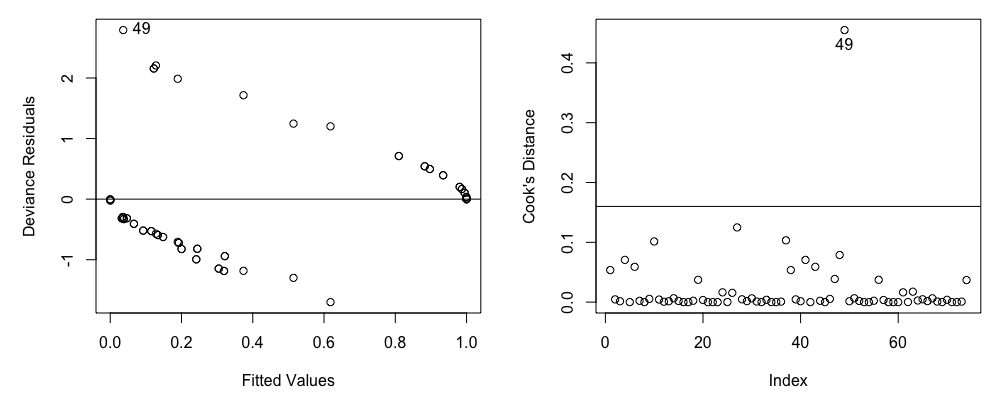
\includegraphics[scale = 0.35]{Rplot49.png}
\caption{On the left, we can see deviance residuals plotted against fitted values, and on the right, we can see Cook's distances  for all data points.}
\end{figure}

We proceed to outlier analysis. As we can see on Figure 3, point 49 has a deviance residual greater than 2 and it has high leverage (as it is far away from other points), and it also has a large influence, as its Cook's distance exceeds the threshold $\frac{8}{n-2p}=0.16$. Therefore it is an outlier and we decide to remove it. 

We fit again model (M4) to a new data set (with point 49 being removed), and we discover that the model is not valid anymore. We receive the warning message signalizing overfitting and all estimates and p-values are extremely small. We decide to remove all three-way interactions, that is we are fitting again model M3 but to a new data set. Estimates look reasonable now, but none of p-values is significant, so this model is also not valid. We decide to remove all interaction terms, that is, we are fitting a model:
\\(M5) growth $\sim$ ph + temperature + nisin + brix 
\begin{table}[h!]
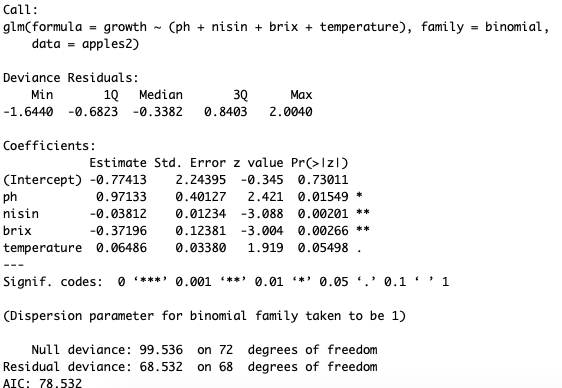
\includegraphics[scale = 0.5]{table9.png}
\caption{Summary of the model (M5) - final model }
\end{table}
\\ 

This model looks plausible, as we can see in Table 9, all terms except temperature are significant at 5\% significance level, and the p-value for temperature is 0.05498, so it is very close to 0.05. We will test if we can drop the temperature from this model. That is, we will compare model (M5) with the model:
\\(M6) growth $\sim$ ph + nisin + brix \\ Model (M5) has residual deviance 68.532  and 68  degrees of freedom, while model (M6) has residual deviance 72.539  and 69  degrees of freedom. Therefore to test if we can drop temperature we compare the LRT statistic 72.539 - 68.532 against chi-squared distribution with 1 degree of freedom. The p-value is 0.045, so it is significant (at 5\% significance level) therefore we will not drop the temperature. Thus, we will use (M5) as our final model. 

\subsection{Outlier analysis}

In Figure 4 we can see four plots that will help us to assess the goodness of fit for our final model. The top left plot presents leverage of each point divided by p/n, as we can see no points are above the threshold 2, so there no points with unusually high leverage, it is a good sign. The top right plot presents deviance residuals, which behave in a way expected for a Bernoulli distribution. The bottom left plot presents the Cook's distance, no point exceeds the $8/(n-2p)$ threshold, so there are no points with unusually high influence, another good sign. And the bottom right plot presents working residuals, everything looks fine. For Bernoulli distribution we cannot expect residuals to be Normal, therefore we have not plotted any qq-plots. 

To summarize, there is no evidence for misfit. The final model fits the data (without point 49) very well. 

\begin{figure}[h!]
\centering
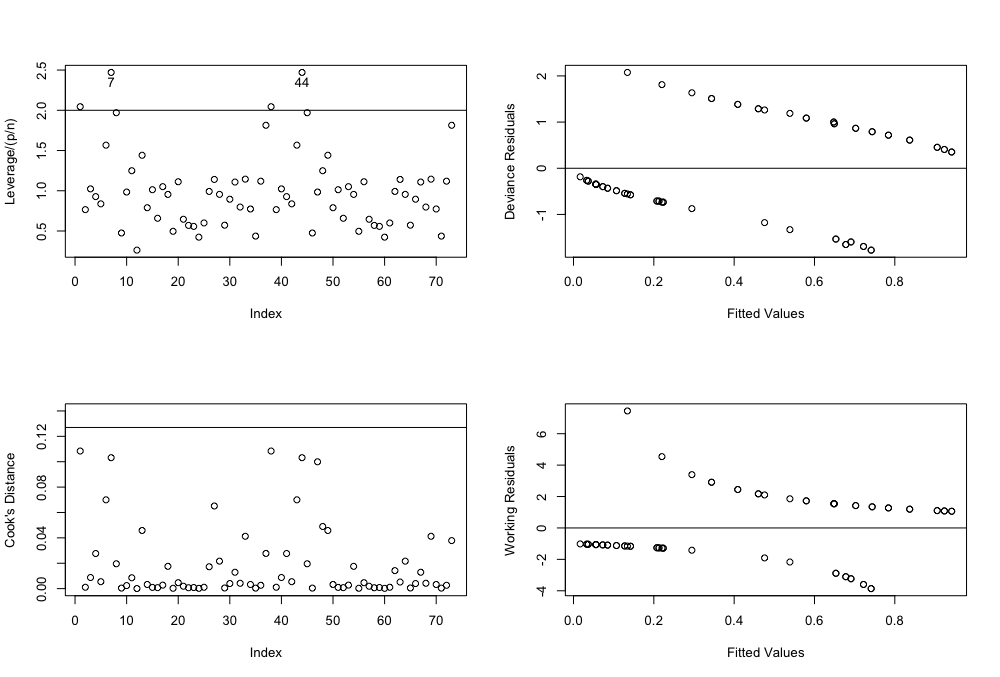
\includegraphics[scale = 0.35]{RplotOut.png}
\caption{Top left plot presents leverage of each point divided by p/n with threshold 2 marked, top right plot presents deviance residuals, bottom left plot presents Cook's distance of each plot and the threshold $8/(n-2p)$, bottom left plot presents working residuals.}
\end{figure}


\subsection{The GLM setup and interpreation}

    The GLM setup for the final model: 
Similarly to the univariate case,  let  \\$y_i=growth[i] $   \\$ \boldsymbol{x_i}=(x_{i,1},x_{i,2},x_{i,3},x_{i,4},x_{i,5})=(1, $ ph$[i],$ brix$[i],$ temperature$[i],$ nisin$[i])$ for $i = 1, 2, ..., 74$\\ Then we model $y_{i} \sim$   Bernoulli($\pi_i$) with $\pi_i$ the probability of growth present, as a function of explanatory variables. The observation model for $y_i$ has following probability mass function:
$$ 
f(y_i|\theta_i,\psi)=\pi_i^{y_i}(1-\pi_i)^{1-y_i}= \exp(y_{i}\log(\pi_i/(1-\pi_i))+\log(1-\pi_i))
$$
so $\theta_i=\log(\pi/(1-\pi)$ is the natural parameter, $\psi=1$, $\kappa(\theta_i = \log(1+e^{\theta_i})$ and $c=0$. We have $\mu_i=E(Y_i)=\pi_i$, and the linear predictor is $\eta_i=\beta_1+\beta_2x_{i,2}+\beta_3x_{i,3}+\beta_4x_{i,4}+\beta_5x_{i,5}$. 
We use the logistic link (which is the canonical link in this case): 
$$
\log(\mu_i/(1-\mu_i))=\eta_i
$$

\subsection{Interpretation of the fitted model}

The estimated change in the log odds when we include the ph term is $\overset{\wedge}{\beta_2} $ = 0.97133, what which is an increase of a factor of exp(0.97133) $\backsimeq $ 2.64.

The estimated change in the log odds when we include the nisin term is $\overset{\wedge}{\beta_3} $ = -0.03812, what which is an increase of a factor of exp(-0.03812) $\backsimeq $ 0.96.

The estimated change in the log odds when we include the brix term is $\overset{\wedge}{\beta_4} $ = -0.37196, what which is an increase of a factor of exp(-0.37196) $\backsimeq $ 0.69.

The estimated change in the log odds when we include the temperature term is $\overset{\wedge}{\beta_5} $ = 0.06486, what which is an increase of a factor of exp(0.06486) $\backsimeq $ 1.07.

\section{Summary}
We have identified point 49 as an outlier and decided to remove it. The best model for this data is growth $\sim$ ph + temperature + nisin + brix. 
\section{Attachments}
R code is attached on the next page. 



\end{document}
